\documentclass[a4paper,12pt]{article} %indique la classe du document, et les options

\pagenumbering{arabic}
%le pr\'eambule

\usepackage[english]{babel}
\usepackage{graphicx}
\selectlanguage{english}

%Titre
\makeatletter
\def\clap#1{\hbox to 0pt{\hss #1\hss}}%
\def\ligne#1{%
\hbox to \hsize{%
\vbox{\centering #1}}}%
\def\haut#1#2#3{%
\hbox to \hsize{%
\rlap{\vtop{\raggedright #1}}%
\hss
\clap{\vtop{\centering #2}}%
\hss
\llap{\vtop{\raggedleft #3}}}}%
\def\bas#1#2#3{%
\hbox to \hsize{%
\rlap{\vbox{\raggedright #1}}%
\hss
\clap{\vbox{\centering #2}}%
\hss
\llap{\vbox{\raggedleft #3}}}}%
\def\maketitle{%
\thispagestyle{empty}\vbox to \vsize{%
\haut{\includegraphics[width=0.35\linewidth]{../../Newcastle-University.jpg}}{\vspace{1cm}\@blurb}{}
\vfill
\vspace{1cm}
\begin{flushleft}
\usefont{OT1}{ptm}{m}{n}
\huge \@title
\end{flushleft}
\par
\hrule height 4pt
\par
\begin{flushright}
\usefont{OT1}{phv}{m}{n}
\Large \@author 
\normalsize \@student
\par
\end{flushright}
\vspace{1cm}
\center
\includegraphics{Metro-Wiki-logo.png}
\vfill
\vfill
\bas{}{\@location, \@date}{}
}%
\cleardoublepage
}
\def\date#1{\def\@date{#1}}
\def\author#1{\def\@author{#1}}
\def\title#1{\def\@title{#1}}
\def\location#1{\def\@location{#1}}
\def\student#1{\def\@student{#1}}
\def\blurb#1{\def\@blurb{#1}}
\date{\today}

\makeatother
\title{
Usability Analysis : \\ Tyne and Wear Metro Ticket machines
}
\author{Nicolas Desfeux}
\student{(Erasmus Student - 110477367)}
\location{Rennes}

\blurb{
Newcastle University\\
\textbf{School of Computing Science}\\[1em]
CSC3003 : Interaction Design
}
%document principal 

\begin{document}
\maketitle
\newpage
\tableofcontents
\newpage
\section*{Introduction}
\addcontentsline{toc}{section}{Introduction}
\paragraph{}The Tyne and Wear is a rail system standing in the North East of England since 1980. Nowadays, this Metro is use for more than 100,000 daily ridership, over sixty stations. To use this Metro, people have to use tickets. In every station, users can find machines that allow them to buy tickets. There is not only one ticket, and several purchase options are available. In this document, we'll first discuss the accessibility and the usability of those machines. Then we'll try to provide a new design, according to the notions we studied in this module.
\section{Usability and accessibility of the Tyne and Wear Metro Tickets machine}
\paragraph{}This section will describe and study the actual tickets machine available in Tyne and Wear Metro stations in Newcastle. The figure \ref{machine} shows you a picture of the actual tickets machine.
\begin{figure}[h!]
\center 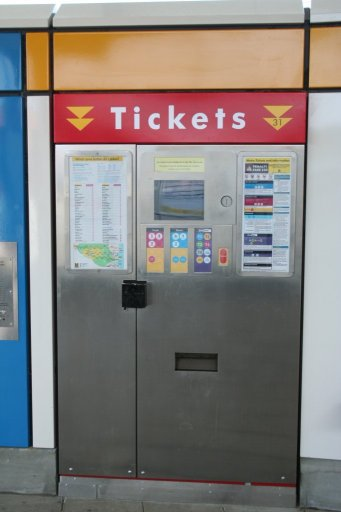
\includegraphics[width=0.35\linewidth]{metro.jpg}
\caption{\label{machine} Tyne and Wear Metro Tickets machine}
\end{figure}
\paragraph{}The machines is kind of a big box, with a screen, some buttons under it, some reading on both sides, a hole to insert coins and a compartment for collecting ticket.
\subsection{Goals}
The purpose of the machine is to provided tickets for the Metro train station. Several kind of tickets are available. There are two options for a ticket : the destination users wants to go, and the validity time of the ticket. The machine might be able to set those options, and provided the good tickets.
\subsection{Usability}
We are now going to analysis the usability of the current machine, using "Dix et al's" usability principles.
\subsubsection{Learnability}
It's easily predictable. Click are followed by screen changes. The buttons' action can be guess. When users knows the system, finding a ticket is always the same method. Function for buttons are quiet familiar. : The shape, the color, suggest that they have to be push. There is a good generalisability, and the system is very consistent : whatever the ticket the user wants to get, it's still the same way of taking it.
\subsubsection{Flexibility}
The flexibility of the system is quiet low. The only freedom user have is the choice of the ticket. After that choice, all actions are give by the system. The system constraint the functionality. On that system, there is no multi-threading.  There is also no substitutivity. The only input user can give are Pound sterling, and the interface is not customizable, which make sense for a ticket machine, as users will normally not have to use it every day.
\subsubsection{Robustness}
The robustness of the system is quiet good. It's easy to see the internal state of the system, as things are displayed on the screen, and each actions are leading to a change on the screen. The recoverability of the system is not very good, as the cancel button bring the display back to the welcome screen. The responsiveness of the system is good. The system is fast, and stable.

\paragraph{} The usability of this machine is quiet unbalanced. Some things are very useful (robustness), are some others are very annoying (payment system).
\subsection{Accessibility analysis}
\subsubsection{Perceptibly}
\paragraph{Information presentation : }All the informations are displayed with text, and colored buttons. There are 3 display zones : 
\begin{itemize}
\item The screen  : The actual screen display informations in two colors : black background, and orange-yellow writing.
\item Metro lines on the left : This shows where the stations are and explains the zones system.
\item General informations on the right : It explains the rules of the rail system, what is allowed and not, ...
\end{itemize}
Under the screen, users can find the buttons for tickets selection.  Buttons are organized to help people easily find the ticket they want.
\paragraph{Assistive technologies} It doesn't seems to have help for people. There is no way to zoom on the screen, and buttons look quiet the same. There is no depth system, for example headphones support, that could help people. Problems subsist also when someone in a wheel chair try to get a ticket. There is no place for a wheel chair to allowed an easy access to every buttons, and payment system. Another, every button shapes are the same, that's not helping someone with eyes disease to find what they want.
\subsubsection{Operability}
\paragraph{Action needed : } To get a ticket, three actions are needed : 
\begin{enumerate}
\item Click on the button corresponding to the ticket users wants to purchase (one of the button below the screen).
\item Insert the coins (and only coins !) corresponding to the price of the ticket.
\item Get the ticket and change from the collecting box, below the buttons.
\end{enumerate}
That's only three actions. The ticket selection might be quiet confusing. To pay for tickets, users can only uses coins. No notes and cards payments are allowed, which can be quiet annoying for the user. The price is displayed on the screen. Theres is no way to get several tickets on the same set of commands. users have to start again to have an other ticket, even if it's the same at the first.

\paragraph{}We also study users input and output : 
\begin{itemize}
\item \textbf{Money}
To put money is the machine, users have to select a ticket first. Otherwise, the pay system is close. The money provider can only be used at the correct time. The only way to put money in is to give coins. The system did not handle cards and notes.
\item \textbf{Collecting box}
We also study users input and output : 
To collect tickets, users have to open a "door" on the machine, where the ticket is released. Most people need to do an extra movement to collect the tickets, and going close to the ground. It's not that easy to see what's in the box when users are standing up.
\end{itemize}
\subsubsection{Simplicity}
The simplicity of this machine is quiet obvious. Just one click to achieve goal. Actions are simple, but users may need some time to do it. For example,  the ticket selection is quiet long if user doesn't know the system.

\subsubsection{Forgiveness}
During the execution of the three action, only the two first need to allow forgiveness. There is, below the screen, a cancel button. If users are executing one of the first two actions, pushing this button cancel everything was begin (remove ticket selection, giving money back if coins was inserted).
\\The pay system is quiet simple too, the price is display on the screen, in a big enough size, and it decrease as user puts money in the machine, to help know how much users still have to put in.

\subsection{Issues summarize}
Even if those machine achieve the goal they are asking for, and some of the design technics used are quiet efficient, there are some issues that we can point out.
Here are some issues that we found about this new machine : 
\begin{itemize}
\item Collecting box position
\item Payment only by cash
\item Screen position and display
\item ...
\end{itemize}

\section{Redesigning  of the Tyne and Wear Metro Tickets machine}
\subsection{Requirement specifications}
The purpose of the ticket machine is to provide tickets for the rail system. Dealing with the good input from the user, the machine have to give a paper ticket, eventually a receipt and some change.\begin{figure}[h!]
\center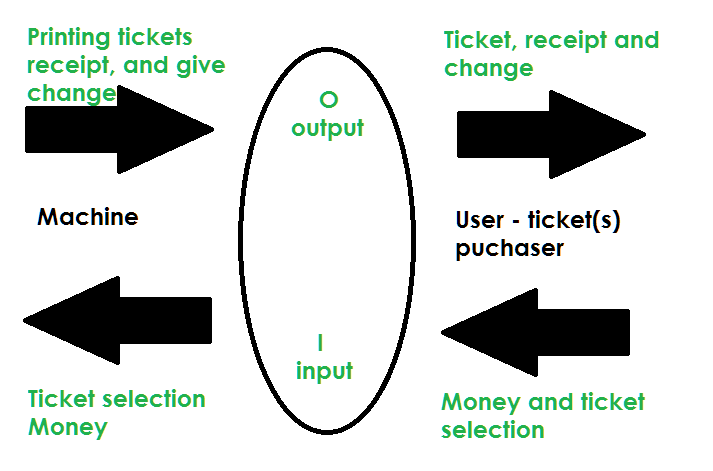
\includegraphics[width=0.75\linewidth]{diagramm.png}
\caption{\label{diagramm}Abowd and Beale diagram}
\end{figure}
\paragraph{}We decided to create a machine divided in three part : 
\begin{itemize}
\item Screen display and user interface
\item Informations
\item Collecting boxes.
\end{itemize}
You can see the overall architecture of the machine we design on the figure \ref{new}.
\begin{figure}[h!]
\hspace{-3.5cm}
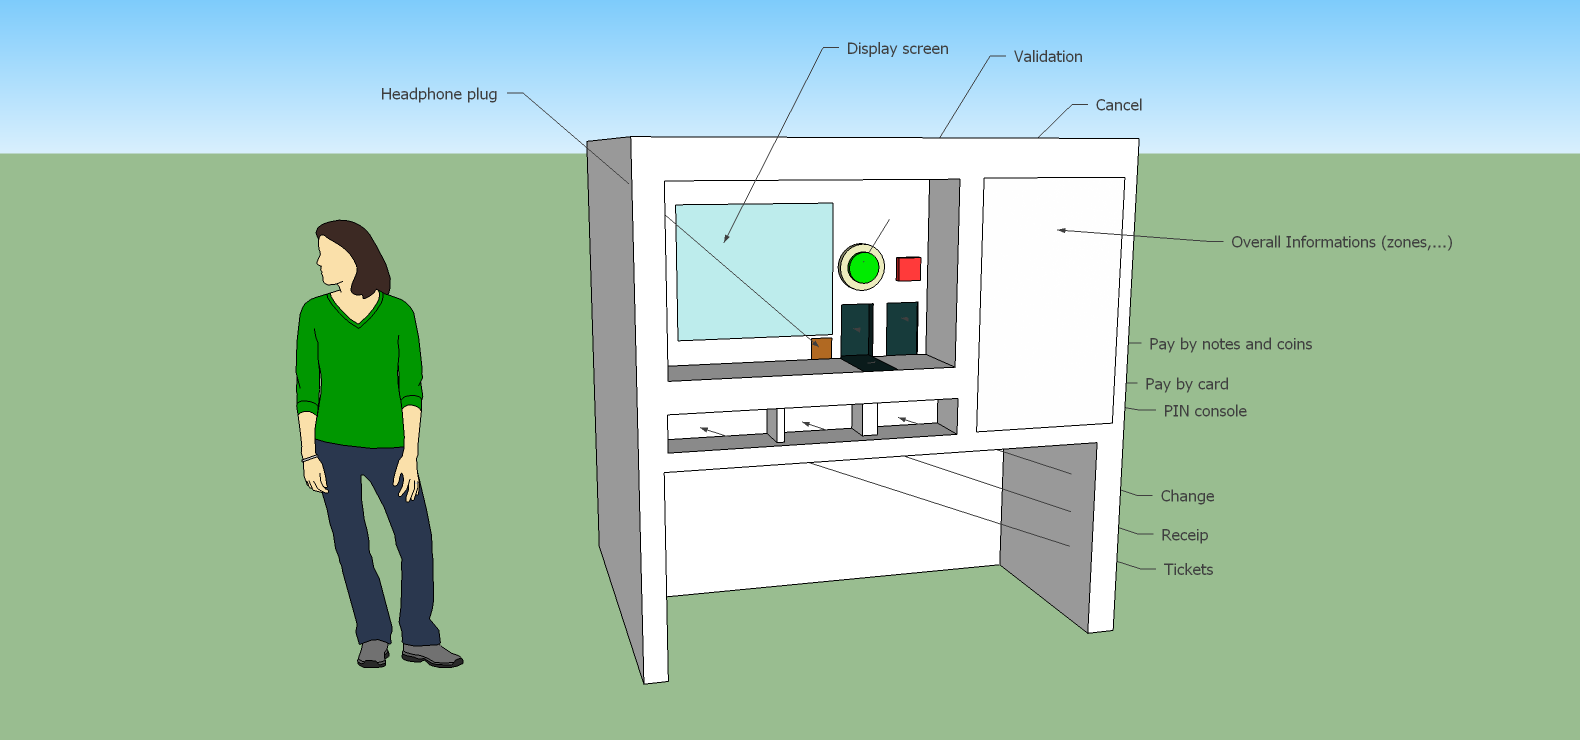
\includegraphics[width=1.5\linewidth]{ID.png}
\caption{\label{new} Tyne and Wear Metro Tickets machine - New design, global view}
\end{figure}
\subsection{Overall description}
We try to create a machine available for every users. There is a space bellow the machine, but make the wheelchair access easier. The screen is not too high. We also provide a small "desk" in front of the machine, to put on wallet on for example. It's useful for people with one hand only for example.  The collecting box is bigger, but it's because more output will be available, compare to the old machine.
\begin{figure}[h!]
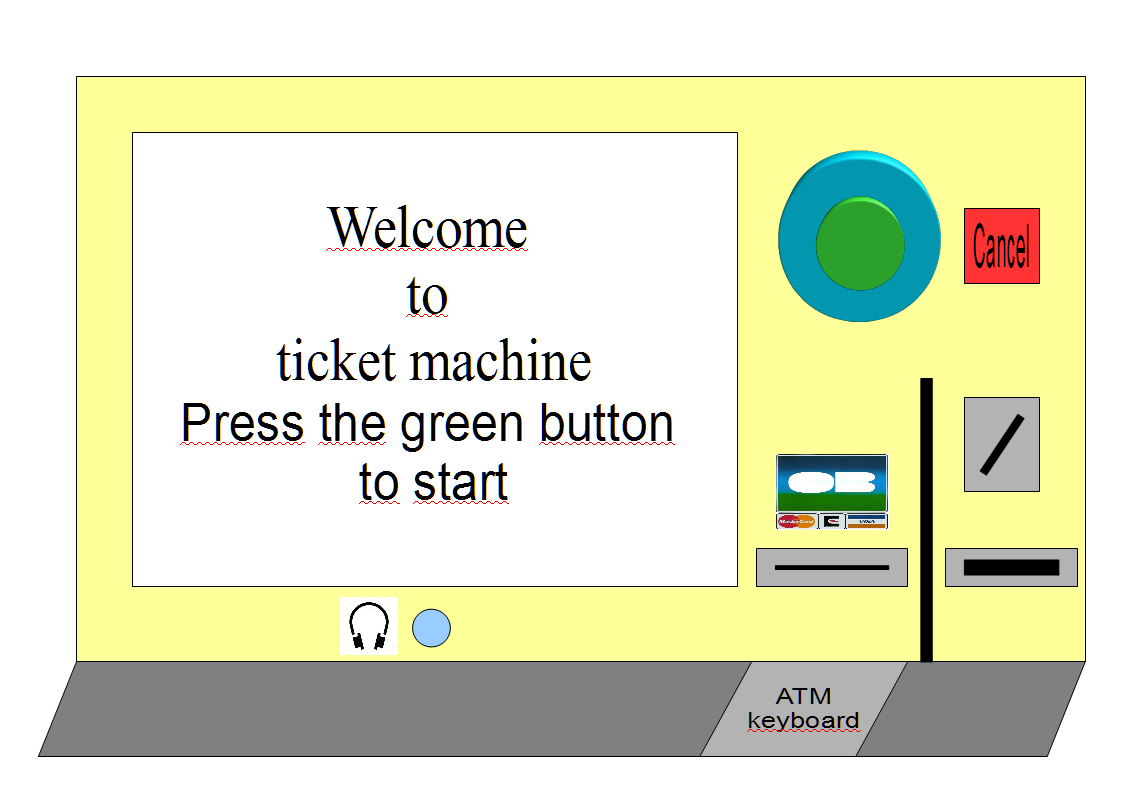
\includegraphics[width=1\linewidth]{interaction1.png}
\caption{\label{userInterface} Tyne and Wear Metro Tickets machine - User interface}
\end{figure}
\paragraph{}We decided to put all the informations (overall rules, zones description,...) on the same side of the machine. By this way, looking for help is going to be easier, as their is only one place to look at. 

\subsubsection{Input}
\paragraph{}
When the user come to purchase tickets, there is two buttons users can use (the green one and the red one on figure \ref{ticket1}): 
\begin{itemize}
\item Green button : There is two kind of action on this button : rotate the button, as a selector, and push, as a validation.
\item Red button : This is the cancel button. He is smaller than the green one, and the shape is not the same.
\end{itemize}
Most of time, users will just have to use the biggest button.

\paragraph{Money input}
We decided to add more payment option, compare to the older machine. We make it possible to use notes and card. The system will be capable of handle the two payment. As user finishes selected tickets, both payment are available. If user insert a card, or cash and notes, only one payment option will stay open.
\begin{itemize}
\item Card : As user validates a ticket selection, card insertion is available. as a card insertion is detected by the system, payment instructions appears on the screen. (reading card in progress, informations, asking for PIN code). The PIN will be enter thanks to a keyboard located just bellow the card insertion location. You can see how it looks like on figure \ref{userInterface}
\item Change : It's now possible to pay using coins and notes. If needed, the system might be able to give change.
\end{itemize}.
\paragraph{Headphone plug}
To help blind people, or people with eye disease, we provide a sound system. The user can activate by plug in a headphone in the design plug in. We isolated that plug, to make it easier to find and use.
\subsubsection{Output}
\paragraph{Screen}
The screen is a colored screen. This is not a touch screen. The screen will provide feed back on the user action. We'll describe later how the screen give that feed back. The screen will also be used for payment options.
\paragraph{Collecting box}
\begin{figure}[h!]
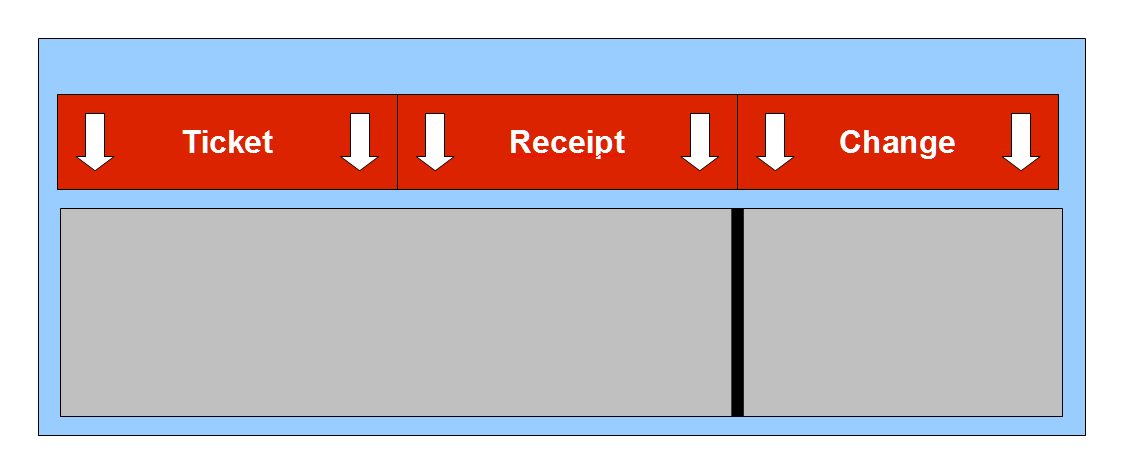
\includegraphics[width=1\linewidth]{interaction6.png}
\caption{\label{ticket6} Collecting box}
\end{figure}
The collecting box is as wide as the machine, and divided in two. On the left compartment, we will collect the ticket, and eventually the receipt if asked. The compartment on the right is used for the change. You can see an idea of what the box looks like in figure \ref{ticket6}
\paragraph{Sounds}
The sound provide in the headphone must describe how to select tickets. Using different shapes for the buttons will be useful to help people with eyes disease to find what they want. The voice should explain what is on the screen, and how to interact with it.
\subsection{Software design}
We are now going to focus on how to purchase a ticket, especially on the screen display. As the user arrive at the machine, it's on a welcome screen (figure \ref{userInterface}). It's just a draw, advertisement could be add for example. This function can also be as an energy saver.
\paragraph{Zone selection}Pushing the green buttons put the machine on. The first screen displayed (figure \ref{ticket1}) is design for zone selection. There are 3 possible choices. To navigate between circles, users the rotative button. Validation is done by pushing the green button. 
\begin{figure}[h!]
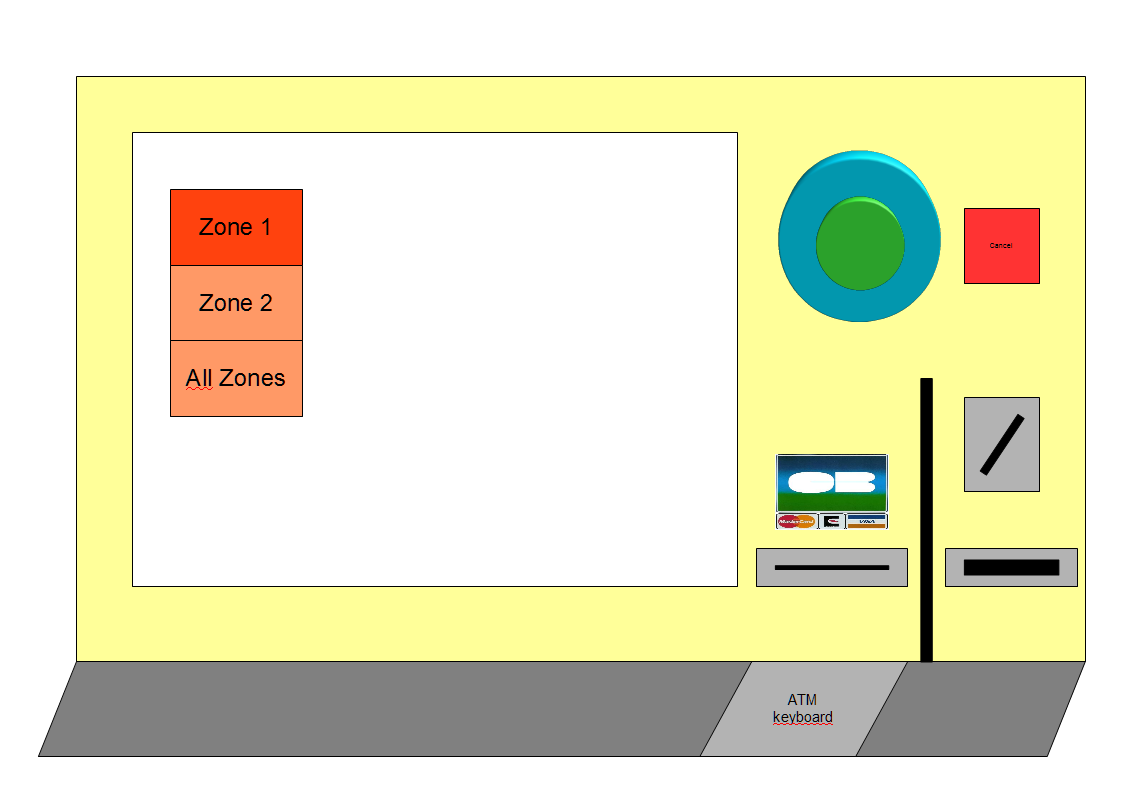
\includegraphics[width=1\linewidth]{interaction2.png}
\caption{\label{ticket1} Tyne and Wear Metro Tickets machine - Zone selection}
\end{figure}
\paragraph{}As the zone is selected, users can selected the type of ticket they want. In case of mistake, user can use the cancel button. We decided to separate every ticket options, user select it one at the time. It made the selection a little bit longer, but more clear.
\paragraph{Quantity selection} 
\begin{figure}[h!]
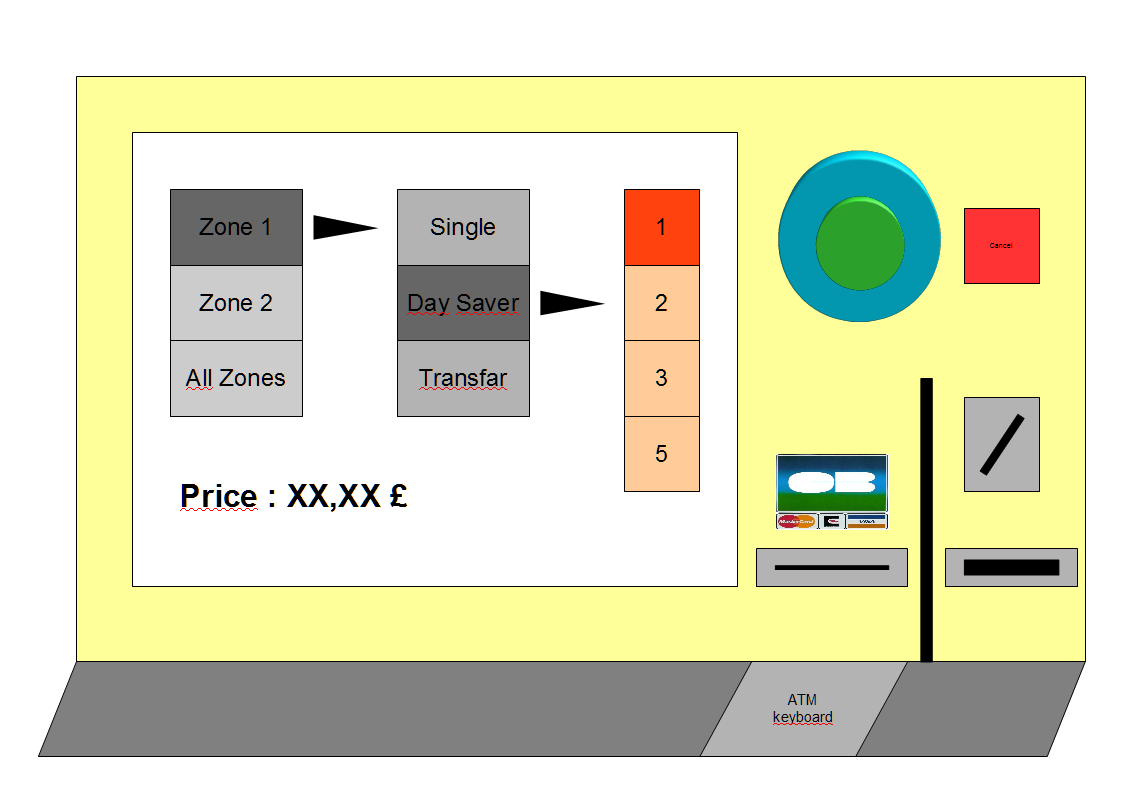
\includegraphics[width=1\linewidth]{interaction4.png}
\caption{\label{ticket2} Tyne and Wear Metro Tickets machine - Quantity selection}
\end{figure}
Users can now buy several tickets at the same time. Selection system is the same as before (rotate the button to select the item, push it to validate). That give the system a consistency for the user. Now that we have enough informations, we are able to display the price, even before the quantity validation. The screen update itself each time user changes the quantity (figure \ref{ticket2}). 
\paragraph{Payment} Once the quantity is validate, the screen display a question for the user, asking if the user needs a receipt. Once the answer is given, payment options become available. At the start, each are available, and once user starts using one of it, the other one close. Screens will help user through it payment. For cash payment, it will show the amount of cash user still needs to insert. If it's a card payment, information relative to it will also be display on the screen (interaction needed with the ATM-like keyboard,...).

\newpage
\section*{Conclusion}
\addcontentsline{toc}{section}{Conclusion}
\paragraph{}The actual metro tickets station that you find in Newcastle clearly have some issues, for classic users (no notes, no cards, ...), and for people with disability (position and size of the machine, no handle of headphones,...). For most of people, those issues are transparent, but they still exist, and some people can have real trouble getting a ticket.
\paragraph{}Designing a new Metro tickets machine is not that easy when you try to fix all of that issue. However, lying on the principle we saw in lectures, we manage to create a machine more usable and accessible for passengers. To be sure of that, the next step would doing an evaluation of this design. The evaluation would help validate (and correct if needed) the design we made. 

\newpage
\listoffigures
\nocite{Org}
\nocite{Wikipedia}
\bibliographystyle{abbrv}
\bibliography{main}
\end{document}